% Standalone render of generated/table_rule_by_strategy.tex
% Build: pdflatex -interaction=nonstopmode rule_by_strategy_standalone.tex
\documentclass{article}
\usepackage[landscape,margin=0.5in]{geometry}
\usepackage{booktabs}
\usepackage{amsmath}
\usepackage{graphicx}
\pagestyle{empty}
\begin{document}
\begin{center}
\textbf{0DTE 15:30--16:00 nearest-OTM straddle: per-rule return summary, models compared on the same 866 days}\\[1.5ex]
% AUTO-GENERATED by writeup/make_rule_by_strategy_tex.py — do not edit.
% Source: results/atm_straddle_0dte_1530/rule_by_strategy_*.csv
\begingroup\small\setlength{\tabcolsep}{3.5pt}
\begin{tabular}{lrrrrrrrrrrrrrr}
\toprule
& $n$ & mean & std & min & 25\% & 50\% & 75\% & max & skew & ex.\ kurt & $t$ & Sharpe$_{\mathrm{ann}}$ & $n_{\mathrm{buy}}$ & \%buy \\
\midrule
\multicolumn{15}{l}{\emph{Short volatility (always short)}} \\
all models (no forecast) & 871 & 0.020 & 1.127 & -10.32 & -0.444 & 0.329 & 0.931 & 1.00 & -2.31 & 10.90 & 0.53 & 0.28 & 0 & 0.0 \\
\midrule
\multicolumn{15}{l}{\emph{$\mathrm{sign}(s)$ ($\pm 1$ on the sign of $s$)}} \\
HAR + calendar OLS & 871 & 0.071 & 1.125 & -5.42 & -0.635 & 0.176 & 0.883 & 10.32 & 0.54 & 10.68 & 1.85 & 1.00 & 280 & 32.1 \\
block-diag ridge & 871 & 0.115 & 1.121 & -5.42 & -0.686 & 0.151 & 0.912 & 10.32 & 0.96 & 10.56 & 3.03 & 1.63 & 339 & 38.9 \\
LightGBM & 871 & 0.094 & 1.123 & -5.42 & -0.639 & 0.176 & 0.900 & 10.32 & 0.90 & 10.58 & 2.48 & 1.33 & 282 & 32.4 \\
XGBoost & 871 & 0.098 & 1.123 & -5.42 & -0.624 & 0.180 & 0.914 & 10.32 & 0.84 & 10.60 & 2.58 & 1.39 & 275 & 31.6 \\
lasso (causally tuned) & 871 & 0.102 & 1.122 & -6.84 & -0.650 & 0.172 & 0.914 & 10.32 & 0.44 & 10.75 & 2.68 & 1.44 & 320 & 36.7 \\
lasso ($\alpha=10^{-4}$) & 871 & 0.130 & 1.120 & -5.42 & -0.698 & 0.124 & 0.892 & 10.32 & 1.29 & 10.42 & 3.42 & 1.84 & 365 & 41.9 \\
elastic net (causally tuned) & 871 & 0.080 & 1.124 & -6.84 & -0.660 & 0.147 & 0.913 & 10.32 & 0.44 & 10.71 & 2.11 & 1.14 & 303 & 34.8 \\
\bottomrule
\end{tabular}
\endgroup

\end{center}
\vspace{1ex}
\begin{center}
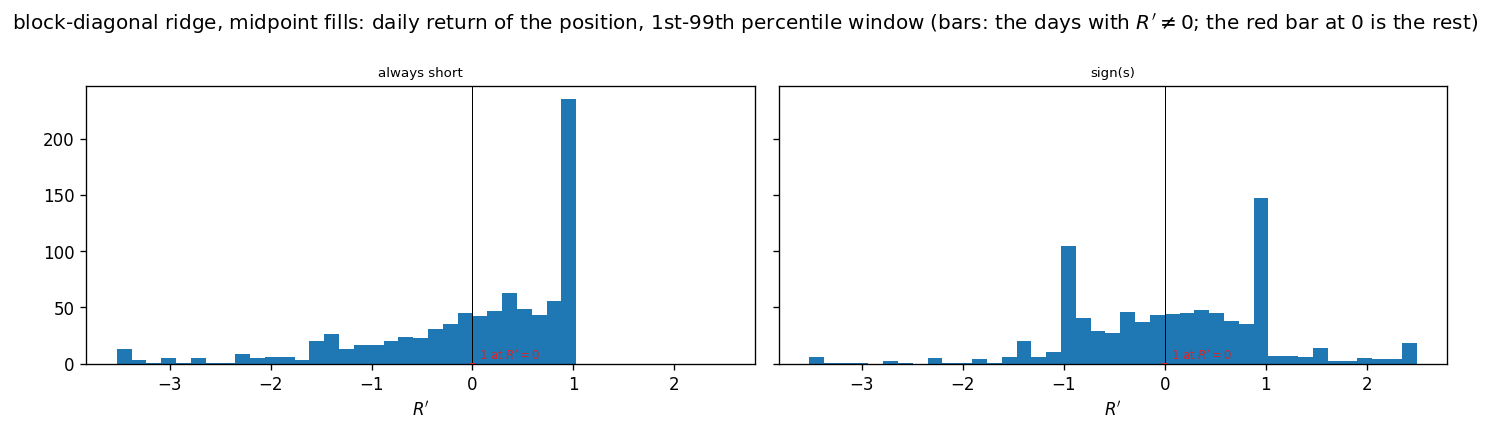
\includegraphics[width=0.85\textwidth]{../results/atm_straddle_0dte_1530/rule_hists_blk2.png}\par\smallskip
\small Distribution of the daily return of the position taken, block-diagonal ridge forecast, one panel per rule
(returns inside their 1st--99th percentile window; the mass at $-1$ is the days the straddle expires worthless).
\end{center}
\vspace{1ex}
\noindent\small \textbf{Straddle} here means the nearest out-of-the-money call plus the nearest
out-of-the-money put, same-day expiry, bought or sold as one position.
One expiration day = one return; mid fill. Every $t$ here is the plain
$t=\sqrt{n}\cdot\mathrm{mean}/\mathrm{std}$, with no autocorrelation correction.
``ex.\ kurt'' is the bias-corrected sample excess kurtosis (Gaussian $=0$).
$n_{\mathrm{buy}}$/\%buy count days the rule is net long ($q_t>0$).
The short-volatility rule takes no forecast, so it is one row for all models.
Sharpe$_{\mathrm{ann}}=(\mathrm{mean}/\mathrm{std})\times\sqrt{252}$; every other column is daily.

\smallskip
\noindent\small Forecasts: baseline (HAR + calendar OLS); block-diagonal ridge (HAR block and exogenous block, separate penalties)
on the design carrying the FOMC calendar block, and the same ridge on the earlier design without those columns, as a diagnostic row;
LightGBM and XGBoost on the all-features design; lasso on the same design, causally tuned vs.\ fixed $\alpha=10^{-4}$;
elastic net (causally tuned). $\dagger$ marks a column still fitted on the earlier design panel; a run of those four on the
panel of record is pending.

\smallskip
\noindent\small \textbf{Per-bar forecasts} (the rows under their own subheading): a separate regression for the 15:30--16:00
bar alone. Each day it is trained on that half hour of the previous 2,000 sessions and nothing else; the target is the
bar's realized variance over its time-of-day baseline, square-rooted; the inputs, all known at 15:30, are each series'
means over the last 1, 5, 25, 125, 625 and 3,125 half-hour bars of the full 24-hour series, is-present flags and calendar
dummies. Ridge penalty chosen from $\{0.01,\ldots,1000\}$ every 250 sessions from past data only (fit on the earlier part
of the window, scored on its last 125 sessions); coefficients re-solved every session; the lasso and elastic net differ
only in the penalty. Column sets: HAR + calendar only; all features; the live-feasible set (16 series a 15:30 forecaster
can rebuild: ES return moments, volume and trade count, VIX, VVIX, VIX3M, the FOMC calendar). The prediction is turned
into a variance by the same recalibration as every other row.
\end{document}
